\subsection{An\'{a}lise Relacionada à Segunda Questão de Pesquisa}


\begin{enumerate}[(QP2)]

\item Quais processos, técnicas ou ferramentas têm sido sugeridos 
na literatura para suportar as atividades de modernização 
dos sistemas legados?

\end{enumerate}

\vspace{0.1cm} 

De modo a facilitar a análise e a resposta desta questão, as publicações foram classificadas em três grupos, de acordo com o seguinte esquema proposto em \cite{Petersen:2008}:

\begin{itemize}

\item \textbf{\textit{Focus Areas} --} São as estratégias de modernização identificadas nas publicações: \textit{Black-box modernization, White-box modernization e Replacement}. Entraram neste grupo todas as publicações que propuseram ou descreveram uma estratégia de modernização, independente de terem sido colocadas em prática.

\item \textbf{\textit{Contribution Type} --} Três tipos de contribuições foram 
identificadas: \textit{Management}, fontes primárias que descrevem algum processo, método ou metodologia de gestão do processo de modernização; \textit{Technical}, publicações que propuseram uma solução ferramental, tais como \textit{frameworks}, bibliotecas de software, barramentos de serviços, entre outros; e \textit{Management and technical}, quando a abordagem descrita na literatura é gerencial e técnica.

\item \textbf{\textit{Research Type} --} Nesta categoria, utilizou-se a classificação proposta em \cite{wieringa2006requirements} para agrupar os tipos de pesquisa refletida nas publicações. 
Conforme pode-se verificar na Figura~\ref{fig:research_type}, 
63.64\% das publicações analisadas são do tipo \textit{Solution Proposal}.

\begin{description}
\item[Solution Proposal.] Uma solução para um problema é proposto, a solução pode ser nova ou uma extensão de uma técnica existente.
\item[Validation.] Investiga as propriedades de uma proposta de solução que ainda não tenha sido implementada na prática.
\item[Evaluation.] As técnicas são aplicadas na prática e uma avaliação da técnica é realizada.
\item[Philosophical Papers.] Publicações que estruturam as pesquisas sobre uma determinada área na forma de taxonomia ou conceitos.
\item[Opinion Papers.] Publicações que expressam a opinião pessoal, sem uma valida\c c\~{a}o emp\'{i}rica.
\item[Experience Papers.] Publicações que explicam sobre uma determinada técnica e como foi feito na prática.
\end{description}

\end{itemize}


Tendo concluído a classificação das fontes primárias, o próximo passo foi gerar o diagrama de bolhas para reportar as frequências 
e distribuições das abordagens de modernização dos sistemas legados identificadas na literatura. 
Esta distribuição resultante pode ser consultada na Figura \ref{fig:buble_diagram}. 

%
% Tipos de pesquisa identificadas nas publicações
%
\begin{figure}
\centering
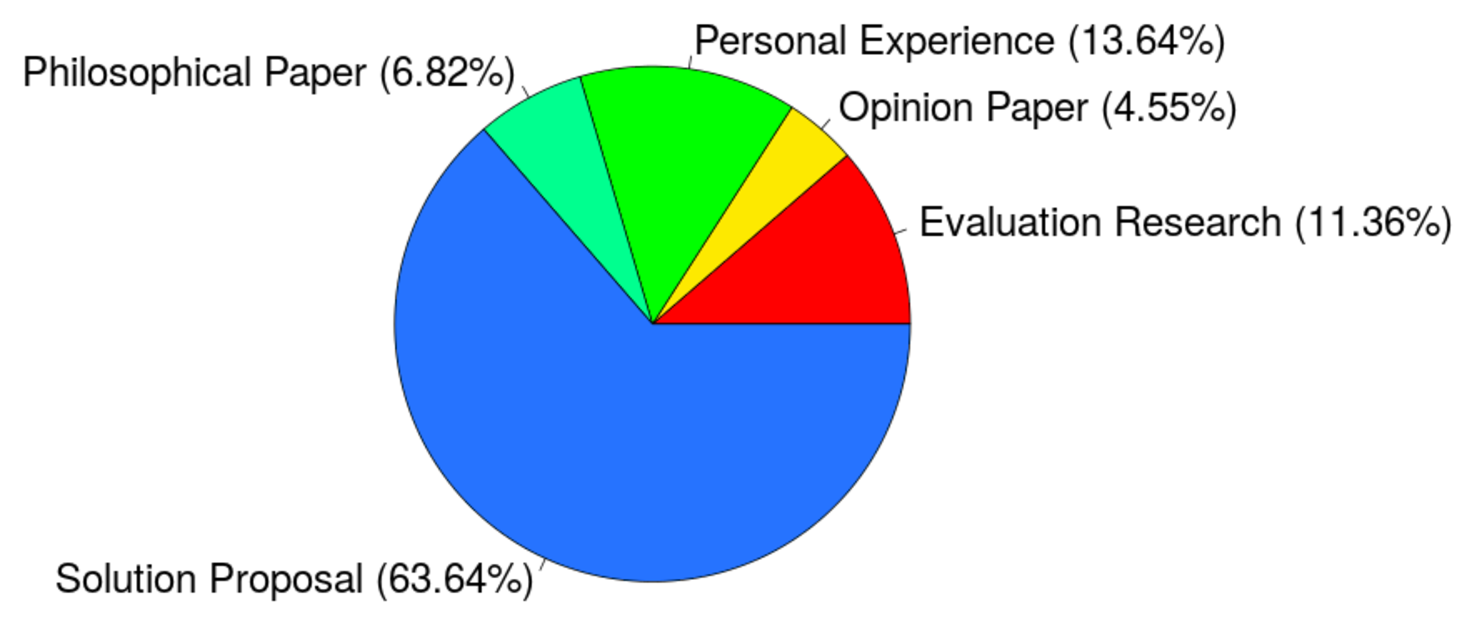
\includegraphics[scale=0.5]{img/mapeamento/research_type.pdf}
\caption{Tipos de pesquisa identificadas nas publicações.}
\label{fig:research_type}
\end{figure}


Como pode-se observar, o diagrama de bolhas exibe uma visão panorâmica dos estudos identificados 
na literatura sobre o tema junto com as lacunas e oportunidades para pesquisas futuras. É possível 
observar que mais de 70\% das pesquisas estão relacionadas com os aspectos gerenciais das atividades de modernização. 
Este cenário, segundo \cite{S13_ransom1998method}, deve-se ao fato da natureza dos projetos de modernização terem que lidar 
com as perspectivas negociais, organizacionais e técnicas ao mesmo tempo. Nesse sentido, um processo de modernização 
pode auxiliar em vários fatores, tais como: decidir se continuam mantendo os sistemas caso os custos ainda sejam justificáveis; 
se uma modernização é a melhor opção ou a substituição é a única alternativa. Além disso, quando a organização já se decidiu 
que a modernização é a única forma de se manter competitiva, é preciso decidir quais estratégias e técnicas de Engenharia de Software são as mais recomendadas 
para cada tipo de sistema. Dessa forma, como afirmam \cite{S05_Lewis:2005, S13_ransom1998method}, a decis\~{a}o 
sobre como deve ser conduzido um projeto de moderniza\c c\~{a}o requer um processo bem definido; incluindo as estratégias de modernização, 
as boas práticas e as recomendações para um gerenciamento efetivo do projeto de modernização. Vários trabalhos têm sido propostos nesse sentido. 
Por exemplo, \cite{S13_ransom1998method} propõem um método de compreensão de um sistema que deve ser executado como primeira atividade em um 
projeto de modernização. Este método fornece um guia para obter as informações necessárias sobre um sistema e a partir daí, permitir selecionar a 
melhor estratégia de modernização baseado nas informações coletadas. Além do mais, no que tange às abordagens utilizadas, 73.52\% faz uso das 
técnicas \textit{White-box} e 23.52\% a \textit{Black-box}. Isso sugere que as técnicas de engenharia de software, como a engenharia reversa, 
são muito utilizadas para obter a compreensão dos sistemas e desenvolver ferramentas para auxiliar na modernização, como foi visto nas publicações
\cite{S29_Chung:2007, S16_fleurey2007model:2007, S13_ransom1998method, S24_visaggio2000value:2000}.


%
% Bubble Plot of the analyzed primary studies
%
\begin{figure}
\centering
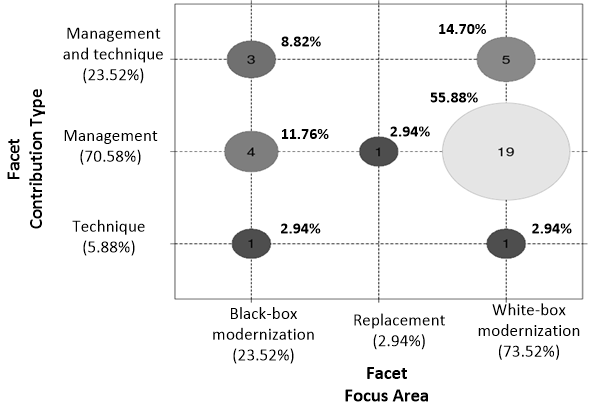
\includegraphics[scale=0.8]{img/mapeamento/bubble_diagram.png}
%\includesvg{bubble_diagram}
\caption{Diagrama de bolhas dos estudos primários analisados.}
\label{fig:buble_diagram}
\end{figure}


% Fim tabela Research Type Facet
% ---------------------------------------------------------------------

\vspace{0.2cm} 
